% TeX
\chapter{无人机引导降落系统研究现状}

 
Kendoul\cite{kendoul2012survey}将无人机系统根据其尺寸、载荷等型号将无人机分为五类。根据本文研究内容的需要,本文将上述类别扩展到固定翼领域。

类别一(Class I):该类别主要指工业和军事领域中的全尺寸无人机系统。这类系统具有较大的载荷、留空时间和工作半径。其典型型号如美国军方的MQ-4C无人机(如图\ref{fig:appendix_03}所示)和波音公司的Unmanned Little Bird (ULB)无人直升机。
%Category I: This category regard to full-scale unmanned
%aircraft. The main feature of this category is their significant
%payload, endurance, and range, but also important the possi-
%bility of carrying a safety pilot on-board the vehicle, thereby
%providing an excellent test bed for complex and risky flight
%tests. The Boeing Unmanned Little Bird (ULB) helicopter and
% MQ-4C Triton are good examples of this category.
\begin{figure}[htb]   
	\centering
	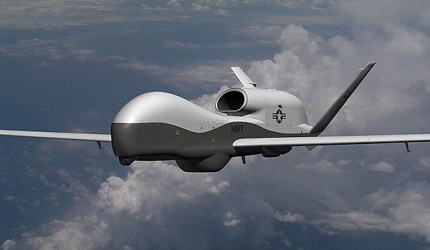
\includegraphics[width=0.5\textwidth]{figs/appendix_03.pdf}
	\caption{MQ-4C}
	\label{fig:appendix_03}
\end{figure}

类别二(CLass II):该类别主要指中等大小尺寸的无人机平台,其有效载荷一般为$10\ kg$以上,起飞重量不小于$30\ kg$,无人机具有完备的自主导航和任务能力。Yamaha RMAX直升机(如图\ref{fig:appendix_02}所示)、德国宇航局的Solar HALE和ELHPSA型固定翼均属于此类别。
%Category II: Medium-scale UAS that are available as
%autonomous or semi-autonomous platforms and have signifi-
%cant payload (more than 10 kg), with a total weight of more
%than 30 kg. Some examples are the Yamaha RMAX, Solar
%HALE(Germany) and ELHASPA (Germany). Different types
%of navigation and mission sensors could be configured on these
%platforms, which are generally well engineered with some level
%of dependability.
\begin{figure}[htb]   
	\centering
	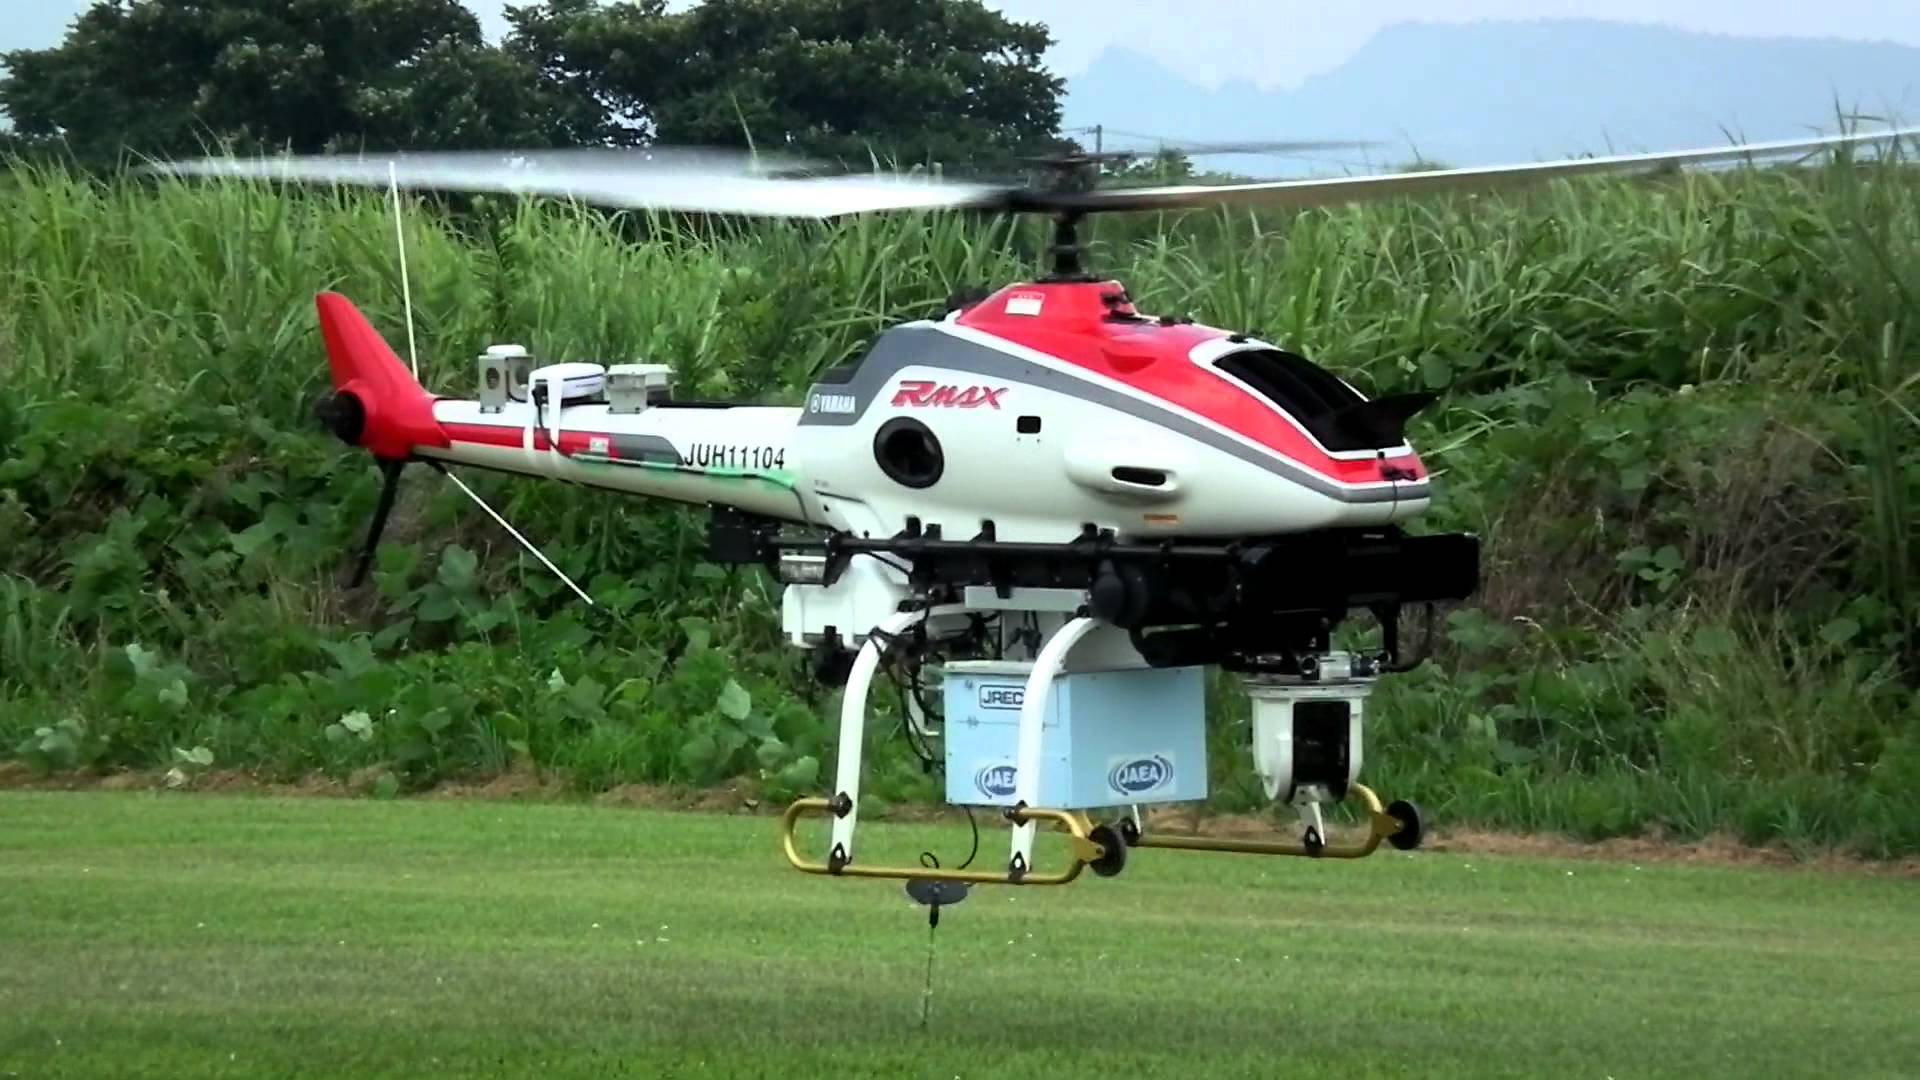
\includegraphics[width=0.5\textwidth]{figs/appendix_02.pdf}
	\caption{Yamaha RMAX直升机平台}
	\label{fig:appendix_02}
\end{figure}

类别三(Class III):该类别的无人机主要指有效载荷在$2\ kg$至$10\ kg$之间的无人机平台,Bergen公司的Vario Benzin Trainer直升机和BAE System的Kingfisher固定翼(如图\ref{fig:appendix_03}所示)均属于此类别。
%Category III: Small-scale UAV are those who have a
%payload of several kilograms (2 to 10 kg) and a total weight
%of less than 30 kg. Helicopters such as the Vario Benzin Trainer
%and Bergen Industrial Twin ; fixed-wing such as AVATAR
%(USA) and Kingfisher (BAE Systems), fall into this category.
%These platforms have less payload than those of Category II,
%but they can still carry most of the navigation and mission
%sensors.

\begin{figure}[htb]   
	\centering
	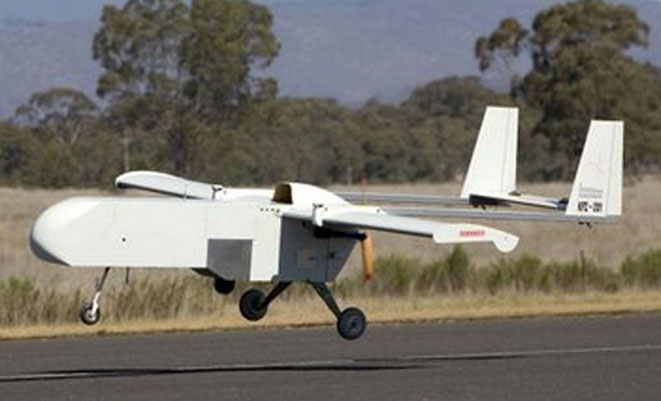
\includegraphics[width=0.5\textwidth]{figs/appendix_01.pdf}
	\caption{Kingfisher固定翼平台}
	\label{fig:appendix_01}
\end{figure}

类别四(Class IV):该类别无人机最为常见,例如大疆的F450系列,德国公司的产品Hummingbird(如图\ref{fig:appendix_04_AscTec_Hummingbird}所示)等。该类型无人机的有效载荷不超过$2\ kg$,主要用于科研单位进行算法的初步测试。由于其有有效载荷重量的约束,这些平台的自主能力受到一定的限制。
%Category IV: Mini-scale UAV that are man-portable
%and can fly outdoors as well as in confined and indoor
%environments. Frog (UAV), DJI NAZA F450 (China), and
%Hummingbird(Germany) and PIXHAWK (Switzerland) fall
%into Category IV, whose payload are generally less than 2 kg
%and total weight can range from hundreds of grams to a few
%kilograms. However, due to the limited payload, only small
%conventional sensors and lightweight sensors are available.
\begin{figure}[htb]   
	\centering
	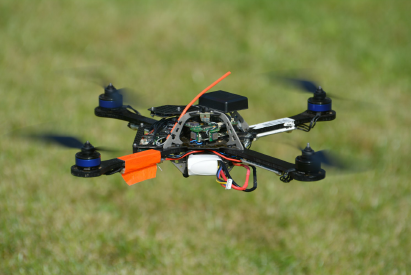
\includegraphics[width=0.5\textwidth]{figs/appendix_04_AscTec_Hummingbird.pdf}
	\caption{AscTec公司的Hummingbird四旋翼平台}
	\label{fig:appendix_04_AscTec_Hummingbird}
\end{figure}


类别五(Class V):这是类别中的最小一类,这类无人机质量一般小于$1\ kg$,例如Seiko Epson的小型无人机系列和PD-100“黑锋”无人机(如图\ref{fig:appendix_05_maxresdefault}所示)。
%Category V: The last category is about micro air vehicles
%(MAVs) with less than 100 g payload, such as the Epson micro
%flying robot, X.R.B helicopter, which are mainly produced for
%indoor research and application. Standard navigation sensors
%and avionics are difficult to carry on these machines.
%B. Motivation for the Scope of This Survey
%Compare with other phases during different automated
\begin{figure}[htb]   
	\centering
	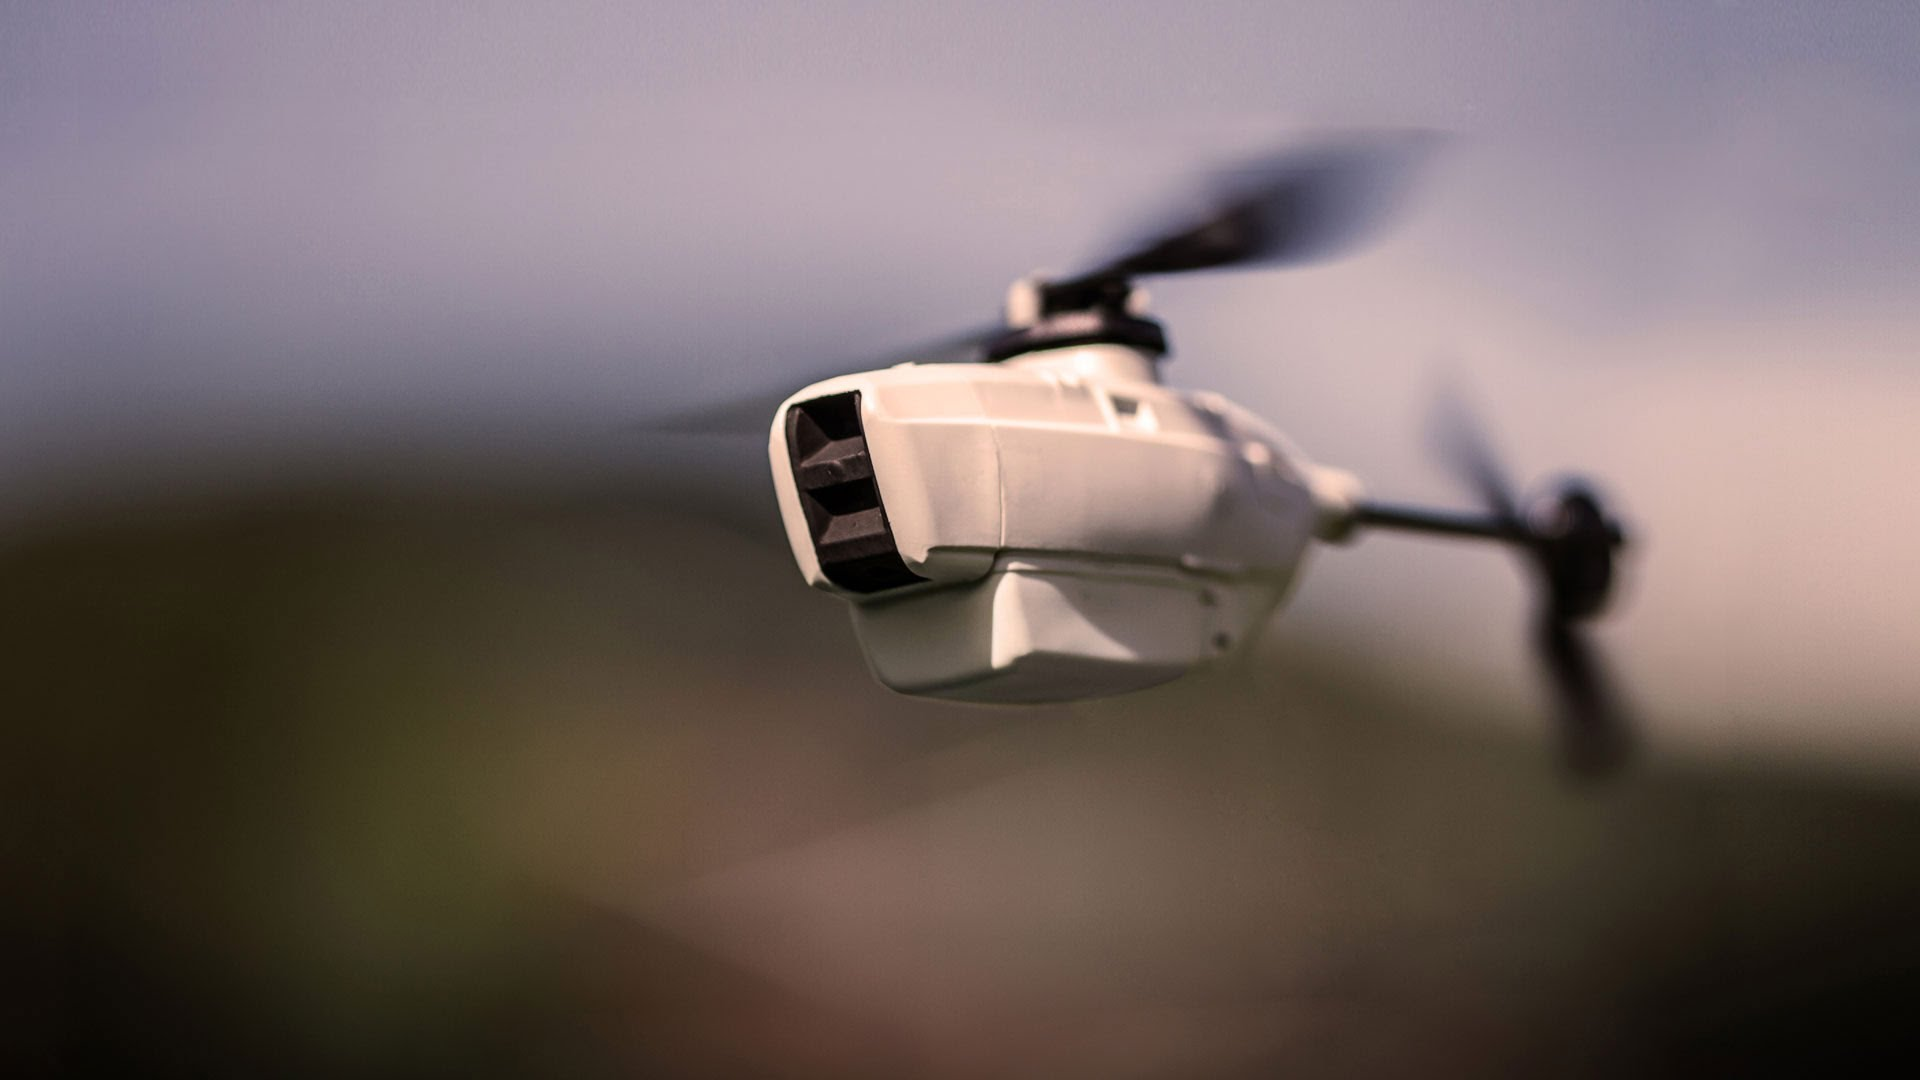
\includegraphics[width=0.5\textwidth]{figs/appendix_05_maxresdefault.pdf}
	\caption{PD-100 无人机平台}
	\label{fig:appendix_05_maxresdefault}
\end{figure}


\begin{landscape}
	\renewcommand{\thefootnote}{\fnsymbol{footnote}}
	\renewcommand{\arraystretch}{0.81}
	\scriptsize
	
	\begin{longtable}{m{5cm}m{5cm}m{5cm}m{5cm}}
		\caption{无人机引导降落系统研究现状}
		\label{table:All_UAV_Research} \\
		
		\hline \hline \\[-2ex]
		\multicolumn{1}{c}{\textbf{研究单位}} &
		\multicolumn{1}{c}{\textbf{无人机平台}} &
		\multicolumn{1}{c}{\textbf{研究领域和项目}} &
		\multicolumn{1}{c}{\textbf{里程碑和主要贡献}} \\[0.5ex]\hline \hline \\[-2ex]
		\endfirsthead
		
		
		\multicolumn{4}{c}{{\tablename} \thetable{} -- Continued}\\[0.5ex]
		\hline \hline \\[-2ex]
		\multicolumn{1}{c}{\textbf{研究单位}} &
		\multicolumn{1}{c}{\textbf{无人机平台}} &
		\multicolumn{1}{c}{\textbf{研究领域和项目}} &
		\multicolumn{1}{c}{\textbf{里程碑和主要贡献}} \\[0.5ex]\hline \\[-2ex]
		\endhead
		
		\multicolumn{4}{c}{{下一页继续}} \\
		\endfoot
		
		\hline\hline\\[-4.0ex] 
		\endlastfoot
		
		\centering German Aerospace Center (DLR), German \cite{Laiacker2013} & \centering \textbf{Class II:} Solar HALE and \textbf{Class II:} ELHASPA & 1. Runway detection methods in different weather and daylight conditions. 2. Multi-sensor automatic landing system. & 1. Increase landing reliability under sub-optimal wind conditions.  2. Adding an additional loop introduced into the altitude controller. \\ 
		\hline
		\centering Universität der Bundeswehr München, German  \cite{Dickmanns1992} & \centering Hardware-in-the-loop simulation & Segmentation of the runway from the substrate.  & 1. The vision system stands alone in manual flight experiments. 2. Combining visual and inertial sensor data evaluation  has complementary beneficial effects.\\ 
		\hline
		\centering University of Central Florida, USA \cite{Miller2008} & \centering  Microsoft Flight Simulator  & The protective geometry of a forward-looking camera. & The system calculate the position of the UAV relative to a known runway by comparing the camera image with a stack of recorded images.\\ 
		\hline
		\centering INRIA Rennes-Bretagne-Atlantique and Institut de Recherche en Informatique et Systèmes Aléatoires (IRISA), France \cite{Rives2002} \cite{Goncalves2011}\cite{Bourquardez2009}\cite{Ozawa2011}& \centering  \textbf{Class IV:} ARMOR X7 and \textbf{Class IV:} Quadrotor  & 1. CIMAR project, IST (Lisboa) project and the Icare Project (INRIA Sophia Antipolis)  2. Position-based visual servoing (PBVS) 3. Image-based visual servoing (IBVS)  & 1. Dynamic Visual Servoing with Image Moments. 2. Dense Visual Tracking method. 3. Design  a suite of image-based kinematic visual servo control schemes to control a quadrotor.\\ 
		\hline
		\centering KAIST, Daejeon, South Korea \cite{Huh2009a} \cite{Kim2014} \cite{Shin2013} \cite{You2012} & \centering  \textbf{Class IV:}  StingRay 60,  \\  \textbf{Class III:} Cessna  172, \\ \textbf{Class IV:} DJI NAZA F450 \\ Matlab\&X-plane simulator & 1. RUAS landing control. 2. Fixed-wing UAS landing control.  & 1. An algorithm for RUAS autonomous landing in crosswind. 2. Line-of-Sight(LOS)-based longitudinal and lateral guidance laws. 3. L1 adaptive control theory for take-off and landing. \\ 
		\hline
		\centering BAE SYSTEMS Australia, Australia \cite{Riseborough2004} & \centering \textbf{Class II:} Kingfisher & Flight control system & A fully autonomous FCS (Flight Control system) \\ 
		\hline
		\centering Santa Clara University, USA \cite{Chatterji1998} & \centering Simulation & Image-based method during night landing. & A vision-based algorithm for estimation of runway relative position (yaw and pitch).  \\ 
		\hline
		\centering University of Southern California, USA \cite{Saripalli2002} \cite{Saripalli2003}\cite{Kelly2008}\cite{Saripalli2007}\cite{Hrabar2003}\cite{Saripalli2003a}& \centering  \textbf{Class III:} AVATAR & 1. Landing UAV on a moving target.  2. Combined Visual and Inertial Navigation. & 1. A trajectory planner based on Variational Hamiltonian and Euler-Lagrange equations. 2. Visual and inertial system without GNSS. \\ 
		\hline
		\centering Department of Electrical Engineering and Computer Sciences, University of California, USA \cite{Sharp2001} \cite{Sinopoli2001}\cite{Shakernia2002}\cite{Sprinkle2005}\cite{Abbeel2010} & \centering  \textbf{Class II:} Yamaha R-50 helicopter and \textbf{Class II:} Synergy N9 & 1. Autonomous helicopter aerobatics control.  2. Vision-based autonomous landing on moving platform. & 1. Apprenticeship learning algorithms. 2. Multiple view motion estimation and control method. 3. Landing path planning based on virtual 3D model.\\ 
		\hline
		\centering Brigham Young University, USA \cite{Barber2009} \cite{Barber2007} & \centering  \textbf{Class IV:} Self-designed fixed-wing UAV & Vision-based landing method. & 1. A vision based landing method for UAVs where a visual marker was used to generate the roll and pitch for flight control. 2. A control method based on optical flow.\\ 
		\hline
		\centering Naval Postgraduate School, USA \cite{Yakimenko2002a} & \centering  \textbf{Class IV:} Frog & UAV shipboard landing. & A shipboard landing method based on infrared camera.\\ 
		\hline
		\centering Australian Defence Science and Technology Organization, Australia \cite{Chahl2004} & \centering Simulation & Bio-inspired landing strategies. & A smooth landing strategy based on optic flow.\\ 
		\hline
		\centering Universite d'Evry, France \cite{Hamel2002} & \centering Simulation & Image-based visual servoing (IBVS). & A new image-based control strategy for visual servoing of a class of under-actuated rigid body systems.\\ 
		\hline
		\centering CEA/LIST Institute, France \cite{Herisse2008}\cite{Courbon2010}\cite{Guenard2008}& \centering  \textbf{Class IV:} X4-flyer & Vision-based navigation strategy. & 1. A nonlinear controller for hovering flight and touchdown control. 2. Build visual path using a single camera by comparing natural landmarks and previous memory.\\ 
		\hline
		\centering The French Aerospace Lab, France \cite{Herisse2012} & \centering  \textbf{Class IV:} Quadrotor & Landing UAV on a moving platform. & A nonlinear controller for vertical landing using optical flow.\\ 
		\hline
		\centering CSIRO Computational Informatics, Australia \cite{Kendoul2013} & \centering  \textbf{Class IV:} Pelican quadrotor & Control method based on the ecological tau theory. & Designed a bio-inspired TauPilot for guidance, navigation and control.\\ 
		\hline
		\centering Virginia Tech, USA \cite{Trisiripisal2006} & \centering  \textbf{Class II:} North American Rockwell OV-10A “Bronco” & Stereo-based autonomous landing method. &  Stereo-based  method for detecting runway edges for estimating distance from the aircraft to the touchdown point.\\ 
		\hline
		\centering Georgia Institute of Technology, USA \cite{Proctor2004} & \centering  \textbf{Class IV:} 2-axis glider & Single vision only method. & The control strategies is capable of flying from a staring point to an ending location using only a single vision sensor.\\ 
		\hline
		\centering ETH Zurich, Switzerland \cite{Meier2011}\cite{Faessler2014} & \centering  \textbf{Class IV:} Pelican quadrotor and \textbf{Class IV:} PIXHAWK Cheetah Quadrotor & 1. Vision-based method in GPS-denied in- and outdoor environments. 2. Visual SLAM algorithm. & 1. PIXHAWK system for autonomous using on-board vision. 2. Mococular-SLAM-based control approach for UAV. \\ 
		\hline
		\centering Linköping University, Sweden \cite{Merz2006} & \centering  \textbf{Class III:} WITAS helicopter & 1.WITAS project. 2. On-board visual navigation system. & Vision only landing method in all weather conditions. \\ 
		\hline
		\centering University of Tuebingen, Germany \cite{Masselli2013}\cite{Yang2012}\cite{Masselli2012}\cite{Wenzel2010a}\cite{Wenzel2010}\cite{Yang2014} & \centering  \textbf{Class IV:} Hummingbird quadrotor and \textbf{Class IV:} PIXHAWK Cheetah Quadrotor & 1.Visual-marker-based landing method. 2. Monocular vision landing system. 3. Visual SLAM. & 1.IR-LED-based landing system. 2. A vision algorithm for estimating 6 DOF of UAV by detecting landing pad. 3. Autonomous landing method based on visual SLAM.\\ 
		\hline
		\centering Università Politecnica delle Marche, Italy \cite{Cesetti2009} & \centering \textbf{Class III:} HELIBOT helicopter  & Autonomous landing without artificial landmark.  & A vision-based gudiance system for navigation and safe landing using natural landmarks. \\
		\hline
		\centering Nanjing University of Aeronautics and Astronautics, China \cite{Xu2009} & \centering  Simulation & Vision-based autonomous landing on a moving ship.  & An autonomous visual landing method based on infrared marker. \\
		\hline
		\centering Beihang University, China \cite{Bi2013} & \centering \textbf{Class IV:} AR.Drone quadrotor  & Autonomous landing of a quadrotor on a moving platform.  & An autonomous visual tracking and landing system. \\
		\hline
		\centering Chinese Academy of Sciences, China \cite{Wu2013} & \centering FlightGear and Matlab simulation.  & Autonomous landing of an unmanned helicopter on a moving ship.  & A path planning method based on linear programming. \\ 
		\centering College of Aerospace Science and Engineering, National University of Defense Technology, China \cite{Gui2013} & \centering \textbf{Class IV:} Self-designed fixed-wing UAV  & Autonomous landing method based on ground visual maker.  & 1. Infrared marker detection algorithm. 2. Vision-based landing method without GNSS.\\
		\hline
		\centering College of Mechatronic Engineering and Automation, National University of Defense Technology, China \cite{Kong2013} & \centering \textbf{Class IV:}  MD4-200 quadrotor and  \textbf{Class IV:} Fixed-wing UAV & Ground-based autonomous landing system.  & A ground-based infrared stereo vision system.\\
		\hline
		\centering Carnegie Mellon University, USA \cite{Scherer2012}\cite{Arora2013} & \centering \textbf{Class II:}   EC 135 helicopter and  \textbf{Class IV:} Bell 206 helicopter & 1. Shipdeck tracking for autonomus landing. 2. Autonomous landing at unprepared sites. & 1. Control strategies for a full-scale helicopter. 2. Vision- and Lidar-based landing methods.\\
		\hline
		\centering Brigham Young University, USA \cite{Barber2007} & \centering \textbf{Class IV:}  Kevlar covered flying wing & Vision-based landing method. & Estimate height above ground (HAG) based on barometric pressure and optic flow. \\
		\hline
		\centering Aix-Marseille University, France \cite{Ruffier2014} & \centering Simulation & Autonomous landing on a moving platform(both vertically and horizontally) based on optical flow. & 1. Design a optic flow regulator. 2. Bio-inspired landing strategies.\\
		\hline
		\centering  Seoul National University, South Korea \cite{Lee2012} & \centering \textbf{Class IV:} Quadrotor & Image-based visual servoing(IBVS). & 1. An adaptive sliding mode controller for landing on a moving target. 2. An IBVS landing algorithm.\\
		\hline
		\centering Universidad Politecnica Madrid, Spain \cite{Garcia-Pardo2002}\cite{Martinez2010}\cite{Martinez2009a} & \centering \textbf{Class III:} Rotomotion SR20 helicopter & 1. COLIBRI Project. 2. Vision-based landing on an unknown place. 3. Image-based visual servoing. 4. Ground-based visual landing system. & 1. A ground-based trinocular visual landing system. 2. An IBVS landing algorithm.\\
		\hline
		\centering  University of Queensland, Australia \cite{Thurrowgood2014}\cite{Yang2011} & \centering \textbf{Class IV:} Super Frontier Senior-46 fixed-wing UAV & 1. A multi-sensor data fusion algorithm. 2. Bio-inspired visual landing system. & 1. A near-panoramic iEye aircraft vision system. 2. A ship-landing algorithm.\\
		\hline
		\centering  University of Florida, USA \cite{Ettinger2002} & \centering \textbf{Class IV:} 6-inch MAV and \textbf{Class IV:} 24-inch MAV & Vision-based control method. & A vision-guided flight stability and autonomy system.\\
		\hline
		\centering  Istanbul Technical University, Turkey \cite{Altug2005} & \centering \textbf{Class IV:} Quadrotor & On-board- and ground-based visual system. & A novel two-camera method is introduced for estimating the full six-degrees-of-freedom pose of the helicopter. \\
		\hline
		\centering  Chiba University, Japan \cite{PEBRIANTI2010}\cite{Yu2010}\cite{Wang2006}& \centering \textbf{Class V:} X.R.B helicopter, \textbf{Class IV:} Quadrotor and \textbf{Class III:} SF40 helicopter & 1. Ground-based visual system. 2. On-board based visual system. & 1. A ground stereo vision system. 2. A single camera with PTU system. 3. A 3 layered landing control framework \\
		\hline
		\centering Boston University, USA \cite{Bosse1998} & \centering \textbf{Class IV:} Quadrotor & Vision-based navigation system. & A vision-based motion estimation method. \\
		\hline
		\centering Ames Research Center, USA \cite{Hubbard2006} & \centering \textbf{Class II:} Yamaha RMAX helicopter & 1. PALACE program. 2. Autonomous landing at unprepared sites. & PALACE automatic control framework. \\
		
		\hline
		
	\end{longtable}
	
	\normalsize
	\renewcommand{\thefootnote}{\arabic{footnote}}
	\renewcommand{\arraystretch}{1.0}
\end{landscape}